\documentclass{sigchi}
% Use this section to set the ACM copyright statement (e.g. for
% preprints).  Consult the conference website for the camera-ready
% copyright statement.

% Copyright
% \CopyrightYear{2016}
%\setcopyright{acmcopyright}
% \setcopyright{acmlicensed}
%\setcopyright{rightsretained}
%\setcopyright{usgov}
%\setcopyright{usgovmixed}
%\setcopyright{cagov}
%\setcopyright{cagovmixed}
% DOI
% \doi{http://dx.doi.org/10.475/123_4}
% % ISBN
% \isbn{123-4567-24-567/08/06}
% %Conference
% \conferenceinfo{CHI'16,}{May 07--12, 2016, San Jose, CA, USA}
% %Price
% \acmPrice{\$15.00}

% Use this command to override the default ACM copyright statement
% (e.g. for preprints).  Consult the conference website for the
% camera-ready copyright statement.

%% HOW TO OVERRIDE THE DEFAULT COPYRIGHT STRIP --
%% Please note you need to make sure the copy for your specific
%% license is used here!
% \toappear{
% Permission to make digital or hard copies of all or part of this work
% for personal or classroom use is granted without fee provided that
% copies are not made or distributed for profit or commercial advantage
% and that copies bear this notice and the full citation on the first
% page. Copyrights for components of this work owned by others than ACM
% must be honored. Abstracting with credit is permitted. To copy
% otherwise, or republish, to post on servers or to redistribute to
% lists, requires prior specific permission and/or a fee. Request
% permissions from \href{mailto:Permissions@acm.org}{Permissions@acm.org}. \\
% \emph{CHI '16},  May 07--12, 2016, San Jose, CA, USA \\
% ACM xxx-x-xxxx-xxxx-x/xx/xx\ldots \$15.00 \\
% DOI: \url{http://dx.doi.org/xx.xxxx/xxxxxxx.xxxxxxx}
% }

% Arabic page numbers for submission.  Remove this line to eliminate
% page numbers for the camera ready copy
% \pagenumbering{arabic}

% Load basic packages
\usepackage{balance}       % to better equalize the last page
\usepackage{graphics}      % for EPS, load graphicx instead
\usepackage[T1]{fontenc}   % for umlauts and other diaeresis
\usepackage{txfonts}
\usepackage{mathptmx}
\usepackage[pdflang={en-US},pdftex]{hyperref}
\usepackage{color}
\usepackage{booktabs}
\usepackage{textcomp}

\usepackage{verbatim}

% Some optional stuff you might like/need.
\usepackage{microtype}        % Improved Tracking and Kerning
% \usepackage[all]{hypcap}    % Fixes bug in hyperref caption linking
\usepackage{ccicons}          % Cite your images correctly!
% \usepackage[utf8]{inputenc} % for a UTF8 editor only

% If you want to use todo notes, marginpars etc. during creation of
% your draft document, you have to enable the "chi_draft" option for
% the document class. To do this, change the very first line to:
% "\documentclass[chi_draft]{sigchi}". You can then place todo notes
% by using the "\todo{...}"  command. Make sure to disable the draft
% option again before submitting your final document.
\usepackage{todonotes}


% === new commands ===
\newcommand\ud{\mathrm{d}}
\newcommand\dist{\buildrel\rm d\over\sim}
\newcommand\ind{\stackrel{\rm indep.}{\sim}}
\newcommand\iid{\stackrel{\rm i.i.d.}{\sim}}
\newcommand\logit{{\rm logit}}
\renewcommand\r{\right}
\renewcommand\l{\left}

\newcommand{\qs}{q^{\star}}
\newcommand{\E}{\mathbb{E}}
\newcommand{\Var}{\mathrm{Var}}
\newcommand{\Cov}{\mathrm{Cov}}
\newcommand{\tr}{\mathrm{tr}}
\newcommand{\1}{\mathbf{1}}
\newcommand{\const}{\mathrm{const.}}
\newcommand{\bx}{\mathbf{x}}
\newcommand{\tbx}{\tilde{\mathbf{x}}}
\newcommand{\ba}{\mathbf{a}}
\newcommand{\bA}{\mathbf{A}}
\newcommand{\bb}{\mathbf{b}}
\newcommand{\bB}{\mathbf{B}}
\newcommand{\bc}{\mathbf{c}}
\newcommand{\bC}{\mathbf{C}}
\newcommand{\bd}{\mathbf{d}}
\newcommand{\bD}{\mathbf{D}}
\newcommand{\bz}{\mathbf{z}}
\newcommand{\bZ}{\mathbf{Z}}
\newcommand{\cN}{\mathcal{N}}
\newcommand{\cG}{\mathcal{G}}
\newcommand{\cI}{\mathcal{I}}
\newcommand{\cIG}{\mathcal{IG}}
\newcommand{\cTN}{\mathcal{TN}}
\newcommand{\balpha}{\boldsymbol{\alpha}}
\newcommand{\bmu}{\boldsymbol{\mu}}
\newcommand{\bSigma}{\boldsymbol{\Sigma}}
\newcommand{\bbeta}{\boldsymbol{\beta}}
\newcommand{\bdelta}{\boldsymbol{\delta}}
\newcommand{\bgamma}{\boldsymbol{\gamma}}
\newcommand{\tbbeta}{\tilde{\boldsymbol{\beta}}}
\newcommand{\bt}{\tilde{\beta}}
\newcommand{\xt}{\tilde{x}}
\newcommand{\Tt}{\tilde{\theta}}
\newcommand{\by}{\mathbf{y}}
\newcommand{\bY}{\mathbf{Y}}
\newcommand{\uT}{\underline{T}}
\newcommand{\oT}{\overline{T}}
\newcommand{\be}{\begin{equation}}
\newcommand{\ee}{\end{equation}}

\newcommand{\blurb}[1]{\footnotesize \flushleft #1}
\newcommand{\pre}[1]{\texttt{#1}}
\newcommand{\R}{\textbf{\textsf{R}}}

\newcommand{\argmax}{\operatornamewithlimits{argmax}}
\newcommand{\argmin}{\operatornamewithlimits{argmin}}










% Paper metadata (use plain text, for PDF inclusion and later
% re-using, if desired).  Use \emtpyauthor when submitting for review
% so you remain anonymous.
\def\plaintitle{Adaptive Engine for MOOC}
\def\plainauthor{Ilia Rushkin}
\def\emptyauthor{}
\def\plainkeywords{Authors' choice; of terms; separated; by
  semicolons; include commas, within terms only; required.}
\def\plaingeneralterms{Documentation, Standardization}

% llt: Define a global style for URLs, rather that the default one
\makeatletter
\def\url@leostyle{%
  \@ifundefined{selectfont}{
    \def\UrlFont{\sf}
  }{
    \def\UrlFont{\small\bf\ttfamily}
  }}
\makeatother
\urlstyle{leo}

% To make various LaTeX processors do the right thing with page size.
\def\pprw{8.5in}
\def\pprh{11in}
\special{papersize=\pprw,\pprh}
\setlength{\paperwidth}{\pprw}
\setlength{\paperheight}{\pprh}
\setlength{\pdfpagewidth}{\pprw}
\setlength{\pdfpageheight}{\pprh}

% Make sure hyperref comes last of your loaded packages, to give it a
% fighting chance of not being over-written, since its job is to
% redefine many LaTeX commands.
\definecolor{linkColor}{RGB}{6,125,233}
\hypersetup{%
  pdftitle={\plaintitle},
% Use \plainauthor for final version.
%  pdfauthor={\plainauthor},
  pdfauthor={\emptyauthor},
  pdfkeywords={\plainkeywords},
  pdfdisplaydoctitle=true, % For Accessibility
  bookmarksnumbered,
  pdfstartview={FitH},
  colorlinks,
  citecolor=black,
  filecolor=black,
  linkcolor=black,
  urlcolor=linkColor,
  breaklinks=true,
  hypertexnames=false
}

% create a shortcut to typeset table headings
% \newcommand\tabhead[1]{\small\textbf{#1}}

% End of preamble. Here it comes the document.
\begin{document}

\title{\plaintitle}

\numberofauthors{3}
\author{%
  \alignauthor{Ilia Rushkin, Glenn Lopez, Andrew Ang, Yigal Rosen\\
    % \affaddr{Notes}\\
    \affaddr{Cambridge, USA}}\\
    % \email{e-mail address}}\\
  % \alignauthor{Leave Authors Anonymous\\
  %   \affaddr{for Submission}\\
  %   \affaddr{City, Country}\\
  %   \email{e-mail address}}\\
  % \alignauthor{Leave Authors Anonymous\\
  %   \affaddr{for Submission}\\
  %   \affaddr{City, Country}\\
  %   \email{e-mail address}}\\
}

\maketitle

\begin{abstract}
  UPDATED---\today. Description of an adaptive recommendation engine for serving assessment questions in a MOOC. Prototype in R exists.
\end{abstract}

% \category{H.5.m.}{Information Interfaces and Presentation
%   (e.g. HCI)}{Miscellaneous} \category{See
%   \url{http://acm.org/about/class/1998/} for the full list of ACM
%   classifiers. This section is required.}{}{}
% 
% \keywords{\plainkeywords}

\section{1. Introduction}
\label{sec:intro}
We would like to create a simple adaptive recommendation engine for an edX MOOC, capable of deciding what item to serve to a user next based on the user's history. Primarily, we are interested in serving assessment items (for this reason, we may use "question" and "item" interchangeably), but instructional materials are also possible. These can be any XBlocks instructional webpages or videos intended to be mixed with assessment items ("if a student has trouble with that question, let them read this" etc.)

We use a variety of Bayesian Knowledge Tracing (BKT) model to estimate the students' state. What makes our situation special is that, as we learned from the adaptive pilot and just generally from seeing MOOCs,

1) Questions in the course differ widely in nature, and in particular in difficulty. Thus, we cannot assign the same values of guess, slip and transit probabilities to them, even if they are all tagged with the same knowledge component.

2) Tagging is complicated: some of the questions are tagged with multiple knowledge components (this is the term we prefer; in other works it is also called "skills" or "learning objectives").

3) In a self-paced MOOC environment, there is a need for a causal structure in the knowledge components: we should not serve to a user items tagged with a knowledge component, if the user has shown lack of knowledge of other knowledge components that are pre-requisite to that one. In the simplest case, it can be dictated by a simple ordered list (the natural order of learning the content of the course), but it could also be a detailed graph of pre-requisite relationships among knowledge components.

4) In a MOOC, the number of students is high, so we can afford to define a model with a large number of parameters and optimize them based on the student interaction data.

\section{2. Related Literature}
\label{sec:lit}
 TBD
 

\section{3. Model Description}
\label{sec:model}
\subsection{Knowledge tracing}
Let there be $Q$ questions in the course ($q=1,2,...Q$), tagged with $N$ knowledge components ($i=1,2,... N$), or KCs for short,  with pre-requisite relationships traced among them. These relations will be involved in the recommendation part of the engine, but not in knowledge tracing. We assume that the mastery of each KC by each course user is a binary latent variable -- the user either has learned it or not -- and we update the mastery matrix $p$, where the element $p_ui$ is the currently estimated probability that the user $u$ has the mastery of the KC $i$. We could define the mastery threshold $p^*\in [0,1]$, and if $p_{ui}\geq p^*$, we say that the mastery of $i$ by the user $u$ is sufficiently certain and no longer needs verification.  We could initialize the mastery probability matrix $p=p^{(0)}$ (students' prior knowledge), after which, when the user has been served a question. When the user submits an answer to the question, it gets a correctness value (score) $C_q^{(u)}\in[0,1]$ and we update the mastery probability of each KC (i.e. this user's row of the matrix $p$). 

The Bayesian updating is easier to write in terms of odds, or even logarithmic odds, rather than the probability $p$: 
\be \mathcal{O}_{ui}=\frac{p_{ui}}{1-p_{ui}},\quad L_{ui}=\log\mathcal{O}_{ui},\quad L^*=\log\frac{p^*}{1-p^*}\label{odds-definition} \ee
So we will translate the transit, guess and slip probabilities into odds as well:
\be o_{qi}^{trans}=\frac{p_{qi}^{trans}}{1-p_{qi}^{trans}},\quad o_{qi}^{guess}=\frac{p_{qi}^{guess}}{1-p_{qi}^{guess}},\quad o_{qi}^{slip}=\frac{p_{qi}^{slip}}{1-p_{qi}^{slip}},\label{odds-params}\ee
Then the update procedure requires defining the likelihood ratios for the case of incorrect (0) and correct (1) answer:
\be x^0_{qi}=\frac{p_{qi}^{slip}}{1-p_{qi}^{guess}},\quad x^1_{qi}=\frac{1-p_{qi}^{slip}}{p_{qi}^{guess}}\label{discrimination}\ee
These matrices encode the relevance of a problem $q$ to an KC $i$. If the problem is irrelevant to a KC, the probability of correct or incorrect score should be independent of that KC. This will be the case if $p_{qi}^{slip}=1-p_{qi}^{guess}$, in which case $x^0_{qi}=x^1_{qi}=1$. We propose to define the relevance matrix, used in the recommendation part of the engine, as:
\be k_{qi}=\log x^1_{qi}-\log x^0_{qi}=-\log o_{qi}^{guess}-\log o_{qi}^{slip}\label{relevance},\ee
a sum of logarithmic odds of non-guessing and non-slipping. While the tagging matrix is binary (a KC is either linked to a question or not), the relevance matrix shows the weight of the link: how much of an evidence for the KC mastery the question provides. The multiplicative factor earned by the mastery odds is:
\be x_{qi}=x^0_{qi}\left(\frac{x^1_{qi}}{x^0_{qi}}\right)^{C_q^{(u)}}\label{increment-factor}\ee
% \be x_{qi}=x^0_{qi}+C_q^{(u)}(x^1_{qi}-x^0_{qi})\label{increment-factor}\ee
For binary (0 or 1) scores, this factor should equal $x^0_{qi}$ or $x^1_{qi}$. How we interpolate between these for fractional scores is a matter of choice. For instance, an alternative definition could be a linear interpolation $x_{qi}=x^0_{qi}+C_q^{(u)}(x^1_{qi}-x^0_{qi})$. We preferred the multiplicative interpolation by looking at the location of the "borderline" score, for which $x_{qi}=1$, reresenting the boundary between correctness and incorrectness. For instance, as a back-of-the-envelope estimate, let the guess and slip probabilities have equal values (typically, they are not too different). In Eq. \ref{increment-factor}, this sets the borderline score at a reasonable 0.5, whereas in case of linear interpolation the borderline score in such a situation equals the slip (= guess) probability, which is likely too low.

The posterior odds, with the evidence of the submitted problem, become $\mathcal{O}_{ui}\to \mathcal{O}_{ui}x_{qi}$. Additionally, we modify the mastery odds due to transfer of knowledge ($p_{ui}\to p_{ui}+(1-p_{ui})p^{trans}_{qi}$), so 
the full update procedure is:
\be \mathcal{O}_{ui}\to o_{qi}^{trans} + (o_{qi}^{trans}+1)\mathcal{O}_{ui}x_{qi}\label{BKT}\ee

This is a type of Bayesian Knowledge Tracing. The main modification is that we allow fractional scores (by means of interpolation) and questions tagged with multiple KCs, so that the parameters carry the index $i$. If a problem is tagged with several KCs ($k_{qi}>0$ for more than one value $i$), we essentially view the problem as a collection of sub-problems, each tagged with a single KC. The predicted odds $\mathcal{O}_{qu}^{predict}$ correct answer by user $u$ on a question $q$ is found as
\be \mathcal{O}_{qu}^{predict}=\prod_i\frac{\mathcal{O}_{ui}(1-p_{qi}^{slip})+p_{qi}^{guess}}{\mathcal{O}_{ui}p_{qi}^{slip}+1-p_{qi}^{guess}},\ee
which is to say that we take the ratio of the probability that each sub-problem is answered correctly to the probability that each sub-problem is answered incorrectly (since we must remove from the ensemble the possibilities of correct answer on some but not all sub-problems). The predicted probability of the correct answer to a problem is found from the odds by the standard transformation as: $\mathcal{O}_{qu}^{predict}/(\mathcal{O}_{qu}^{predict}+1)$.

The outlined procedure is multiplicative in nature. A natural idea would be to replace it with an additive one by working with logarithmic odds $L_{ui}$, which we do in the recommendation part of the engine. It would be clearly preferable from the computational point of view in the knowledge-tracing part as well, if it was not for the knowledge-transfer step: in the additive formulation this step would involve an exponentiation and a taking a logarithm.

For terminological simplicity we referred to the content items as questions. However, the model can accomodate instructional items as well, e.g. videos or text. We can adopt a rule that, if an item $q$ is instructional, the outcome of user's interaction with it is always "correct". A way to think of it is to imagine that $q$ includes an assessment part of trivial difficulty. The slip probabilities $p_{qi}^{slip}=0$, the guess probabilities now have the meaning of the probability of not learning an KC from the item, and so we set them to $p_{qi}^{guess}=1-p_{qi}^{trans}$. Also, in case of an instructional item, unlike an assessment item, we may or may not want to mark it as "seen", because it is allowed to serve it to a user multiple times (or perhaps we should impose a limit on how many times it can be served).

If the matrix $p$ or other parameter matrices contain zeros or ones it is possible to encounter $0/0$ indeterminacies. One way to preclude these is adopt a small cutoff, e.g. we can set $\epsilon=10^{-10}$, and make all elements of the parameter matrices $p^{slip},p^{guess},p^{transit}$, as well as the initial mastery probability $p^{(0)}$, be in the interval $[\epsilon,1-\epsilon]$.

\subsection{Recommendation part}

The strategy we use for recommending the next item is a weighted combination of four sub-strategies. Each sub-strategy comes in with an importance weight (the vector of these weights is a governing parameter of the adaptive engine). In particular, if we want to eliminate one sub-strategy, we can simply set its weight to 0. When the user has requested

The pre-requisite relationships among the KCs are naturally visualized as a directed acyclic graph, and is stored as an $N\times N$ matrix $w$ of pre-requisite strengths, $w_ij$ representing the strength of the graph edge from KC $j$ to KC $i$ ($j$ is a pre-requisite for $i$). We define this strength to be on the scale from 0 to 1. If there are no connections, $w$ a zero matrix.

For each KC and for each user, we can define the pre-requisite readiness:
\be
r_{ui}=\sum_{j=1}^{N}w_{ij}\min\left(0,L_{uj}-L^*\right). \label{readiness}
\ee

An element $r_{ui}$ has value 0 if the user has sufficiently mastered all KCs pre-requisite for the KC $i$, and less than 0 if the matery probabilities for some pre-requisites are not yet certain. If the pre-requisite strength $w_{ij}$ is weaker, it enters $r_{ui}$ with a smaller weight, in a sense allowing less certain mastery of less important pre-requisites. If all the pre-requisites are ascertained, $r_{ui}=0$, otherwise it is less than 0. We can deviate from this slightly and introducing a forgiveness parameter $r^*\geq 0$, we assume that a user $u$ is sufficiently ready for learning an KC $i$ if $r_{ui}+r^*\geq 0$. If $r^*>0$, it means that we "forgive" some degree of uncertain knowledge of pre-requisites.

To recommend the next question for a student, we subset the matrix $k_{qi}$ to only those questions (matrix rows) that belong to the current homework and that a user $u$ has not seen yet. Thus, we obtain a user specific matrix $k_{qi}^{(u)}$. We define the non-negative user-specific vectors of "remediation", "continuity", "preparedness", and "difficulty appropriatness" (in terms of difficulty level of the problem $d_q\in[\epsilon,1-\epsilon]$):
\be
R_q^{(u)}=\sum_{i=1}^N k_{qi}^{(u)}\max\left(0,L^*-L_{ui}\right)
\ee
\be
C_q^{(u)}=\sqrt{\sum_{i=1}^N k_{qi}^{(u)}k_{q_{last},i}},
\ee
\be
D_q^{(u)}=-\sum_{i=1}^N k_{qi}^{(u)}\left|L-\log\frac{d_q}{1-d_q}\right|
\ee
\be
P_q^{(u)}=\sum_{i=1}^N k_{qi}^{(u)}\min(0,r_{ui}+r^*)
\ee
where $q_{last}$ is the last item the user saw.
\footnote{We leave an option to bring them all to scale by normalizing each vector with non-zero range to range 1:
\be
R_q^{(u)}\to\frac{R_q^{(u)}}{\max(R_q^{(u)})-\min(R_q^{(u)})},\quad \textrm{and similar for others},
\ee
where it is understood that the renormalization is performed only if the denominator is not 0.}

These expressions are invented, they can be modified in many ways. More competing considerations can be added to the list at will. The idea is that we want to maximize some linear combination of them. As defined here, $P_{q}^{(u)}\leq 0$, $R_{q}^{(u)}\geq 0$, $D_{q}^{(u)}\leq 0$. A larger remediation value for a question means that this question focuses on those KCs for which the user's probability of mastery is currently low. We introduce a vector of importance weights $W=(W_r,W_c,W_d,W_p)$ (defined up to normalization) which measures the relative importance of each: the next item $q$ to serve should be the one which maximizes the combination $W_rR_q^{(u)}+W_cC_q^{(u)}+W_dD_q^{(u)}+W_pP_q^{(u)}$. 

The serving stops naturally in two cases: if we exhausted the available questions (the matrix $k^{(u)}$ has no rows) and 2) if $R_q^{(u)}=0$ for all $q$, which means that the user has reached the mastery threshold $p^*$ on all KCs relevant for the available questions. Additionally, we may or may not adopt the policy that questions with zero remediation value (i.e. mastery threshold reached for all tagged KCs) should not be served ("stop on mastery").

\section{4. User experience}
We use an LTI tool, multiple instances of which can be plugged in as adaptive modules in different parts of the course. E.g. at the end of each course chapter there is an assessment module. The instance of the LTI tool (referred to as "LTI box") is a frame with navigation controls, inside which an edX Xblock of an item is iframed. Once the user submitted the item (if the item has a submit button, i.e. it is a question), clicking on "Next Item" causes the next item to be iframed, and so on, creating a service sequence of items. The adaptivity means that the length and the order of items in the sequence are personalized. The same item cannot be served to a user more than once.
\begin{figure}[t]
\centering
  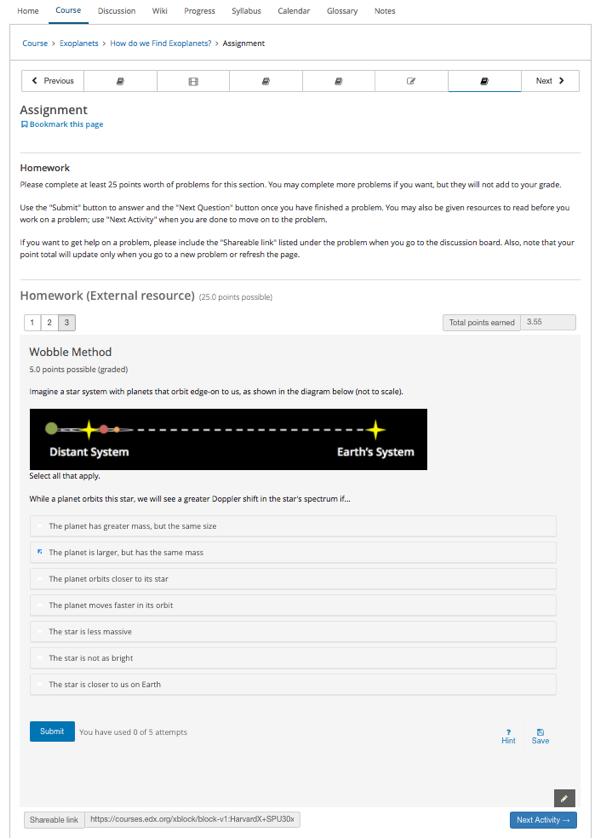
\includegraphics[width=1\columnwidth]{lti-tool}
  \caption{Appearance of an LTI box in a course. At top of the box there is a navigation bar, user can freely move along the instantiated service sequence of items. At the bottom is the button for requesting to continue the sequence and a shareable link to the currently displayed item, so it can be used, for example, in forum discussions.
 }~\label{fig:lti-tool}
\end{figure}
The adaptive engine maintains a knowledge profile for each user, i.e. the estimated personal probability of mastery on each knowledge components. The user's knowledge profile is updated after every submit event by that user (including the submits that happen outside the LTI tool). However, the user's also need to be assigned a score for an adaptive assessment module. Such a score should be calculated in a way that looks fair and clear to the users, regardless of the differences in the personalized service sequences. The situations is easier when all questions assigned to one adaptive module are worth equal number of points. For each module, we set the minimum number of questions $Q$ that we would like a user to do. Then, if $p$ is the number of currently earned points in the module and $q$ is the number of distinct items submitted (i.e. multiple submit attempts on the same item count as 1),
\be \textrm{score}=\left\{
\begin{matrix}
\frac{p}{Q} & \textrm{ if }q<Q\textrm{ and sequence not over}\\
\frac{p}{q} & \textrm{ otherwise}
\end{matrix}
\right.
\ee
Each adaptive module comes with its own bank of items. I.e. a question may be served in adaptive module 1 but not in adaptive module 2. But we also allow for a special category of items that can be served in any adaptive module, they just need to be marked as belonging to this type by the course developing team.

Students in the course will be split randomly into three groups in the 1/1/1 ratio. Group C will not experience adaptivity at all - these students will get the existing non-adaptive version of the course, nothing to do with what we are describing in this work. The other two groups, A andB, will experience adaptivity. The "stop-on-mastery" policy will not be implemented for either group (we do not refuse to serve a question on whose KCs the user's mastery probability exceeds $p^*$). In group A, $W_r=2$ and $W_c=1$ (i.e. remediation has higher importance than continuity). In group B this is reversed: $W_r=1$ and $W_c=2$. The other importance weights are the same for both groups: $W_d=0.5, W_p=1$. 


\section{5. Optimization of BKT parameters}
\label{sec:optimization}
We will rely on a way to optimize our BKT parameters, inspired by the "empirical probabilities" method of \cite{hawkins2014learning}.

At some point in time, when we decide to run the optimization, suppose that the items submitted by a user $u$ are $\{q^{(u)}_j\}$ ($j=1,...J^{(u)}$), indexed in chronological order. Let the correctness of answers be $C^{(u)}_{j}$. We denote $K^{(u)}_{ij}$ this student's knowledge of an KC $i$ just before submitting the item $q^{(u)}_j$. Assuming that there is no forgetting, the knowledge is a non-decreasing function with values 0 and 1, so it is characterized simply by the position of the unit step: for $j$ from 1 to some $n_i$ knowledge is 0 and from $n_i+1$ onward it is 1. We find which $n_i$ gives the highest accuracy of predicting correctness from knowledge. The generalized number of errors on predicting the outcome based on mastery of a particular knowledge component are:
\be E^{(u)}_i(n)=\left(-\sum_{j=1}^{n}C^{(u)}_j\log o^{guess}_{q_j,i} - \sum_{j=n+1}^{J^{(u)}}(1-C^{(u)}_j)\log o^{slip}_{q_j,i}\right),\ee
where $n\in[0,J^{(u)}]$ and we adopt the convention that if the lower limit of a sum is greater than the upper limit, the sum is 0. We set the knowledge step where it minimizes the errors:
\be n_i=\argmin(E^{(u)}_i),\ee
and construct the step-function $K^{(u)}_{ij}$ using it $n_i$. If there are multiple equal minima, and so multiple $n_i$, we take the average of the corresponding multiple step-functions (because of this, knowledge may now have fractional value). The resulting $K^{(u)}_{ij}$ is our empirical estimate of the knowledge of all KCs by the user $u$. Repeat the procedure for each user. Note that, if user's problems are irrelevant for an KC, we will find a steadily growing knowledge of that KC. This is not bad, however, since for each KC we will average only over the users who experienced some relevant problems. Namely, we can define the sets of users
\be
\mathcal{U}_i=\{\forall u: \sum_{j=1}^{J^{(u)}}k_{q_j^{(u)},i}>\eta\},
\ee
\be
\mathcal{U}_{qi}=\{\forall u: \sum_{j=1}^{J^{(u)}}k_{q_j^{(u)},i}\1(q^{(u)}_j=q)>\eta\}
\ee
where $\eta\geq 0$ is a constant we set as a measure of how much total relevance of a KC is enough for the user to be included into the ensemble for estimating the parameters of that KC. As the simplest choice, $\eta=0$.

Since the order of items was chronological, $K^{(u')}_{i,1}$ estimates the prior knowledge of concepts by that user. Moreover, we can identify the occasions when slips, guesses or transfers of knowledge occured. Averaging these over the users we get the empirical matrices of prior knowledge, transit, guess and slip probabilities as ratios:
\be\label{emp.prior} P^{(0)}_{u'i}=\frac{\sum_{u\in\mathcal{U}_i}K^{(u)}_{i,1}}{\sum_{u\in\mathcal{U}_i}1}\ee
(same priors for all users $u'$, i.e. all rows of $P^{(0)}$ are identical)
\be\label{emp.trans} P^{trans}_{qi}=\frac{\sum_{u\in\mathcal{U}_{qi}}\left(\sum_{j=1}^{J^{(u)}-1}(1-K^{(u)}_{ij})K^{(u)}_{i,j+1}\1(q^{(u)}_j=q)\right)}{\sum_{u\in\mathcal{U}_{qi}}\left(\sum_{j=1}^{J^{(u)}-1}(1-K^{(u)}_{ij})\1(q^{(u)}_j=q)\right)}\ee
\be\label{emp.guess} P^{guess}_{qi}=\frac{\sum_{u\in\mathcal{U}_{qi}}\left(\sum_{j=1}^{J^{(u)}}(1-K^{(u)}_{ij})C^{(u)}_{j}\1(q^{(u)}_j=q)\right)}{\sum_{u\in\mathcal{U}_{qi}}\left(\sum_{j=1}^{J^{(u)}}(1-K^{(u)}_{ij})\1(q^{(u)}_j=q)\right)}\ee
\be\label{emp.slip} P^{slip}_{qi}=\frac{\sum_{u\in\mathcal{U}_{qi}}\left(\sum_{j=1}^{J^{(u)}}K^{(u)}_{ij}(1-C^{(u)}_{j})\1(q^{(u)}_j=q)\right)}{\sum_{u\in\mathcal{U}_{qi}}\left(\sum_{j=1}^{J^{(u)}}K^{(u)}_{ij}\1(q^{(u)}_j=q)\right)}\ee
Here again, we adopt the convention that if the lower limit of a sum is greater than the upper limit, the sum is 0 (this happens when $J^{(u)}$ is 0 or 1). The value of the denominator in each of these expressions is a measure of how much student information we have for estimating the probability. In case there is no data, the expression becomes a 0/0 indeterminancy. We should not want to update a probability in this case. Moreover, we impose a threshold $M$ (e.g. 20) and say that we will not update a particular probability if the denominator in the corresponding equation is less than $M$. This is simple to enforce in practice: add to eqq. (\ref{emp.prior}, \ref{emp.trans},\ref{emp.guess},\ref{emp.slip}) the rule that in each of them the denominator less than or equal to $M$ (this roughly counts the number of terms in the denominator sum) should be replaced by 0. After that, any non-numeric (indeterminate or infinite) elements of the matrices $P^{(0)}$, $P^{trans}$, $P^{guess}$, $P^{slip}$ should be replaced by the corresponding elements of the matrices $p^{(0)}$, $p^{trans}$, $p^{guess}$, $p^{slip}$.

We should also watch out for guess and slip probabilities of 0.5 and up. If this happens, we will not update with such values.

Now we can update the BKT parameter matrices with the estimates: $p^{(0)}=P^{(0)}$, $p^{trans}=P^{trans}$, $p^{guess}=P^{guess}$, $p^{slip}=P^{slip}$, and also convert probabilities to odds, i.e. $L^{(0)}_{ui}=\log(p^{(0)}_{ui}/(1-p^{(0)}_{ui})$, and the guess, slip, transit odds via (\ref{odds-params}).

In addition to that, we should also update some elements of the current mastery odds $L$. Namely, let us call "pristine" those elements of $L$, which have never been updated with a non-zero shift via (\ref{BKT}). All the pristine elements of should be replaced with the corresponding elements of $L^{(0)}$. This way, the optimized prior KC knowledge values will be used for all users yet to come to the course, but also for the existing users for those knowledge components that they have not yet explored.

\section{6. Model parameters}
\label{sec:params_smes}
As described in section \ref{sec:model}, the model is governed by the following constants: the mastery threshold $L^*$ (maybe 2.2, corresponding to 0.9 probability), the pre-requisite forgiveness parameter $r^*$ ( maybe 0), the vector of relative importances of recommendation sub-strategies $W$ and the regularization cutoff $\epsilon$ (maybe $10^{-10}$). In addition, as will be described in section \ref{sec:optimization}, there are threshold for updating BKT parameters: $\eta$ (maybe 0) and $M$ (maybe 20).


The minimal information we need from the course developer or SME is

1. Item tagging (which item  is tagged with which KC or KCs).

2. Item placement (which item should be served in which adaptive module; or belongs to the type servable in any module).

3. Item worth (which item is worth how many points). Note that the grading strategy we have currently demands equal point worth in all items that could be served in the same module. But this might change in the future.

4. Pre-requisite relations among knowledge components (at its simplest, the learning order of KCs, which KC should be learned before which). If this is not provided, the engine will assume that no pre-requisite relations exist and so will not use that as a factor in the recommendation decision. 

More information is useful but not strictly required, so can be provided partially or not at all: probabilities of guessing (correct despite not knowing KC), slip (incorrect despite knowing KC)  and transfer (learning KC from doing the item) per item per tagged KC. If we have a cold start, we start with cold guesses for all these parameters in the knowledge tracing, until enough user transactions are accumulated to replace these values with the estimates from the data. By default, the cold start parameters are the same across all questions, but if SME provides the information of this type, we can use it.

% To form the matrix $w$, we require an SME to produce the pre-requisite relationship graph of knowledge components, indicating the strength of the relations. Realistically, we expect the SMEs to use three distinct values of strength: "none" (the absence of the edge in the graph), "weak" and "strong", and we will then convert these to numeric values adopting some convention (e.g. "none"=0,"weak"=0.5, "strong"=1). How complex a graph the SME produces will vary strongly. But at a minimum, we should have a chain of knowledge components indicating the order in which they should be learned.
% 
% To form the matrices $p^{guess}, p^{slip}$, $p^{trans}$, we require an SME to tag each content item with relevant KCs, indicating the level of relevance of each. From these, we will form the tagging matrix $T_{qi}$ (1 if question $q$ is tagged with KC $i$ and 0 otherwise), and the relevance information will be used to populate the values of the guess, slip and trans matrices. Where the tagging matrix has a 0, the guess and slip probabilities are set to 0.5, and the transit probability is set to 0. Higher relevance values means lower guess and slip probabilities. We could also ask SME to indicate guess, slip and transit probabilities severally, by asking questions such as "On the 0-10 scale, how likely is it to solve this problem correctly despite not knowing the KC?" 
% 
% Once we have a substantial amount of student data, we will optimize them (section \ref{sec:optimization}).


\section{7. Testing predictive power of knowledge tracing}
We used the data from the HarvardX course Super-Earths v3 for testing the predictive power of the knowledge-tracing algorithm. The problems in this course tagged with 66 KCs by SMEs. Unfortunately, the number of problems was disproportionately small for this many KCs. 22 of the KCs had only one problem associated with them, 18 KCs had 2 problems, 13 KCs -- 3 problems, 8 KCs -- 4 problems, 2 KCs -- 5 problems, 3 KCs -- 7 problems. So we cannot expect much, but we want to at least see that nothing crazy happens when problems are tagged with more than 1 KC. Restricting ourselves to KCs with more than 3 problems (13 KCs) leaves 60 problems, 3 of which are tagged with 2 KCs, with 2,362 users attempting them, a total of 56,178 submits. Alternatively, we tagged the items using an automated procedure. In this case the KCs are much better populated with problems (here, too, we dropped some KCs with too few problems, but this was insignificant). This gives us a data set with 133 problems, 2837 users, 19 KCs, and a total of 172,410 submits. This automated tagging did not contain multiple KCs per item.

For both taggings, we performed a 3-fold validation, splitting the list of users randomly into thirds, cyclicly using two of them as the training set and the remanining third as the validation set. To alleviate the random effect of some users having significantly more submits than others, we repeated the 3-fold procedure 10 times. Thus, we are calculated the accuracy measures from a vector of observed submit correctnesses and a vector of predicted submit correctnesses, and the length of each vector is 10 times the number of submits in our data set, i.e. 561,780 for SME-tagged data and 1,724,100 for auto-tagged data.

The algorithm was optimized with parameters $\eta=0$, $M=20$. We use five measures of prediction quality: the negative logarithmic likelihoods (total $-LL$, and also separately $-LL_{+}$ for correct and $-LL_{-}$ for incorrect answers; high $-LL_{+}$ is a sign of many false negatives, and high $-LL_{-}$ is a sign of many false positives), as well as the mean absolute error (MAE) and the root-mean-square error (RMSE):
\be -LL=-\frac{1}{2\log 2}\left(\frac{1}{|N|}\sum_{i\in N}x_i\log p_i +\frac{1}{|N|}\sum_{i\in N}(1-x_i)\log (1-p_i)\right)\ee
\be -LL_{+}=-\frac{1}{2\log 2}\left(\frac{1}{|N_+|}\sum_{i\in N_+}\log p_i\right)\ee
\be -LL_{-}=-\frac{1}{2\log 2}\left(\frac{1}{|N_-|}\sum_{i\in N_-}\log (1-p_i)\right)\ee
\be MAE=\frac{1}{|N|}\sum_{i\in N}|x_i-p_i|\ee
\be RMSE=\sqrt{\frac{1}{|N|}\sum_{i\in N}(x_i-p_i)^2},\ee
where the notation is: $N$ is the set of question-user records, divided into the set $N_+$ of correct responses and the set $N_-$ of incorrect responses. The correctness of each question is $x_i=0,1$ and $p_i$ is the predicted probability of correct response. Thus, larger value of $-LL_{+}$ means underestimating correctness (trend to false negatives), and larger value of $-LL_{-}$ means overestimating correctness (trend to false positives). As defined, all measures would equal 0.5 if prediction were done by a coin toss, and 0 if prediction was perfect ($x_i=p_i$). As a performance benchmark, we take the "mean-trained chance" prediction with $p_i$ being the mean correctness in the training set (same value for all problems).

% 2) "specific chance" -- an improved version, where $p_i$ is the problem-specific mean correctness in the training set (different for each problem), but that's tough to beat.

\begin{table}[ht]
\caption{SME-tagged data (561,780 predictions).}
\centering
\begin{tabular}{c c c}
\hline\hline
  & knowledge tracing & mean-trained chance\\ [0.5ex] % inserts table %heading
\hline
$-LL$ & 0.420 & 0.476 \\
$-LL_{+}$ & 0.436 & 0.335 \\
$-LL_{-}$ & 0.394 & 0.715 \\
MAE & 0.330 & 0.467 \\
RMSE & 0.447 & 0.483 \\ [1ex]
\hline
\end{tabular}
\label{tablesme}
\end{table}

\begin{table}[ht]
\caption{Auto-tagged data (1,724,100 predictions).}
\centering
\begin{tabular}{c c c}
\hline\hline
  & knowledge tracing & mean-trained chance\\ [0.5ex] % inserts table %heading
\hline
$-LL$ & 0.379 & 0.366 \\
$-LL_{+}$ & 0.319 & 0.166 \\
$-LL_{-}$ & 0.612 & 1.142 \\
MAE & 0.295 & 0.326 \\
RMSE & 0.428  & 0.404 \\ [1ex]
\hline
\end{tabular}
\label{tableauto}
\end{table}
We see that the knowledge tracing always substantially outperforms prediction by coin-toss (which would have all five accuracy measures equal to 0.5). For the SME-tagged data knowledge tracing outperforms the prediction by mean-trained chance. The latter method simply always predicts that the answer will be correct. The only measure which is lower for the chance prediction is $-LL_{+}$, but that is inconsequential: indeed, since this method always predicts the outcome "correct", it has no false negatives at all. For the auto-tagged data, knowledge tracing outperforms prediction by mean-trained chance only according to MAE. But even if it loses to the mean-trained chance, it is valuable simply because it is adaptive: we could not base a recommendation engine on a prediction method which simply always predicts the same outcome.

If we predict correctness by rounding the probability of correctness (i.e. predicted correctness value is the more likely one of the two), we can see the confusion matrices (Tables \ref{confsme} and \ref{confauto}).
\begin{table}[ht]
\caption{SME-tagged data (561,780 predictions). Accuracy (sum of diagonal terms in the confusion matrix) is 69.4\% for knowledge tracing and 62.9\% for mean-trained chance.}
\centering
\begin{tabular}{c c c}
\hline\hline
{\bf knowledge tracing} & observed $-$ & observed $+$\\ [0.5ex] % inserts table %heading
\hline
predicted $-$ & 28.7\% & 23.3\% \\
predicted $+$ & 8.5\% & 39.5\% \\ [1ex]
\hline
\end{tabular}
\begin{tabular}{c c c}
\hline\hline
 {\bf mean-trained chance} & observed $-$ & observed $+$\\ [0.5ex] % inserts table %heading
\hline
predicted $-$ & 0\% & 0\% \\
predicted $+$ & 37.1\% & 62.9\% \\ [1ex]
\hline
\end{tabular}
% \begin{tabular}{c c c}
% \hline\hline
%  {\bf special chance} & observed $-$ & observed $+$\\ [0.5ex] % inserts table %heading
% \hline
% predicted $-$ & 14.2\% & 8.95\% \\
% predicted $+$ & 19.2\% & 57.60\% \\ [1ex]
% \hline
% \end{tabular}
\label{confsme}
\end{table}
\begin{table}[ht]
\caption{Auto-tagged data (1,724,100 predictions). Accuracy (sum of diagonal terms in the confusion matrix) is 74.6\% for knowledge tracing and 79.5\% for mean-trained chance.}
\centering
\begin{tabular}{c c c}
\hline\hline
{\bf knowledge tracing} & observed $-$ & observed $+$\\ [0.5ex] % inserts table %heading
\hline
predicted $-$ & 10.4\% & 17.7\% \\
predicted $+$ & 10.1\% & 61.7\% \\ [1ex]
\hline
\end{tabular}
\begin{tabular}{c c c}
\hline\hline
 {\bf chance} & observed $-$ & observed $+$\\ [0.5ex] % inserts table %heading
\hline
predicted $-$ & 0\% & 0\% \\
predicted $+$ & 20.5\% & 79.5\% \\ [1ex]
\hline
\end{tabular}
\label{confauto}
\end{table}


\section{8. Automated content tagging}

!!!

This section is a placeholder and although the details of the auto-tagging method have changed, it has not been updated here. 

!!!

Tagging items with KCs is a laborious task for SMEs, so automation, even a partial one, is welcome. If SME tagging is unavailable, we can rely on the automated tagging. If not, automated tagging may serve as the starting point and guidance in the SME's tagging work.

We experimented with the possibility of using a natural language processing algorithm called STM (structural topic model) for this purpose. The textual content of a number of documents is viewed as a mixture of a number of topics, which are defined by the probabilities with which each word is employed. The number of topics is an input to the STM algorithm, which identifies the topics via an optimization technique. As an output, we obtain the  topic properties (how common is each word in a topic), and a non-negative prevalence matrix $\theta_{qt}$, which shows the weight ("prevalence") of a topic $t$ in a document $q$. The normalization is $\sum_{t}\theta_{qt}=1$ for any $q$. We can adapt this model to the tagging task. The documents are the questions (items) and the topics are the knowledge components. An item $q$ is considered tagged with a KC $i$, if the value $\theta_{qi}$ is high enough: we set a threshold $\theta^*$, and the tagging matrix is $T_{qi}=\1{\theta_{qi}>\theta^*}$. If $\theta^*=0.5$, each item will be tagged with at most one KC, apart from the rare possibility of a tie between two KCs, but lower threshold makes multiple-KC tagging possible. To guarantee no untagged items, set $\theta^*\leq\min_q\max_i\theta_{qi}$. If STM is used solely on the basis of the item texts, it reduces to the correlated topic model (CTM). The advantage of STM is that it can include the item metadata as covariates. For instance, the section number, to which an item belongs in the course, may be an important covariate for tagging. Comparing such single-KC tagging with the human tagging of 39 problems from the Super-Earths v3 course, we found Cramer's V coefficient\footnote{A measure of similarity for categorical variables, between 0 and 1, an analog of correlation for quantitative variables.} >0.4.

What number of KCs to use may be left for SME to decide, but as a guidance, we can ask for the "clearest tagging", by which we mean that the prevalences of the tagged KCs should be high: 
\be N=\argmax\left(\frac{1}{N'}\sum_{q=1}^{N'}\max_{i}\theta^{(N')}_{qi}\right),\ee
where the upper index in $\theta$ indicates that this matrix is the output of the STM with $N'$ topics. This describes the unsupervised automated tagging. The supervised version uses pre-existing tagging of some items and extends it to all. In the simplest version, it will not expand the list of KCs. This can be achieved by training a classifying random forest (with the KCs as the response variable) on the pre-tagged items. 


\section{9. Conclusion}
We thank Rob Rubin, Gregory Weber, Liberty Munson, Doipayan Roy and Krishna Madhavan for stimulating discussions.
\label{sec:conc}



% BALANCE COLUMNS
\balance{}

% REFERENCES FORMAT
% References must be the same font size as other body text.
\bibliographystyle{SIGCHI-Reference-Format}
\bibliography{bkt_bibliography}


\end{document}
